\item A tábua de \SI{25}{\kilogram} está suspensa pelas cordas em $C$ e $D$. Se essas cordas estão submetidas a forças constantes de \SI{150}{\newton} e \SI{225}{\newton}, respectivamente, determine a aceleração inicial do centro da tábua e sua aceleração angular. Suponha que a tábua seja uma placa fina. Despreze a massa das polias em $E$ e $F$.

\begin{flushright}
	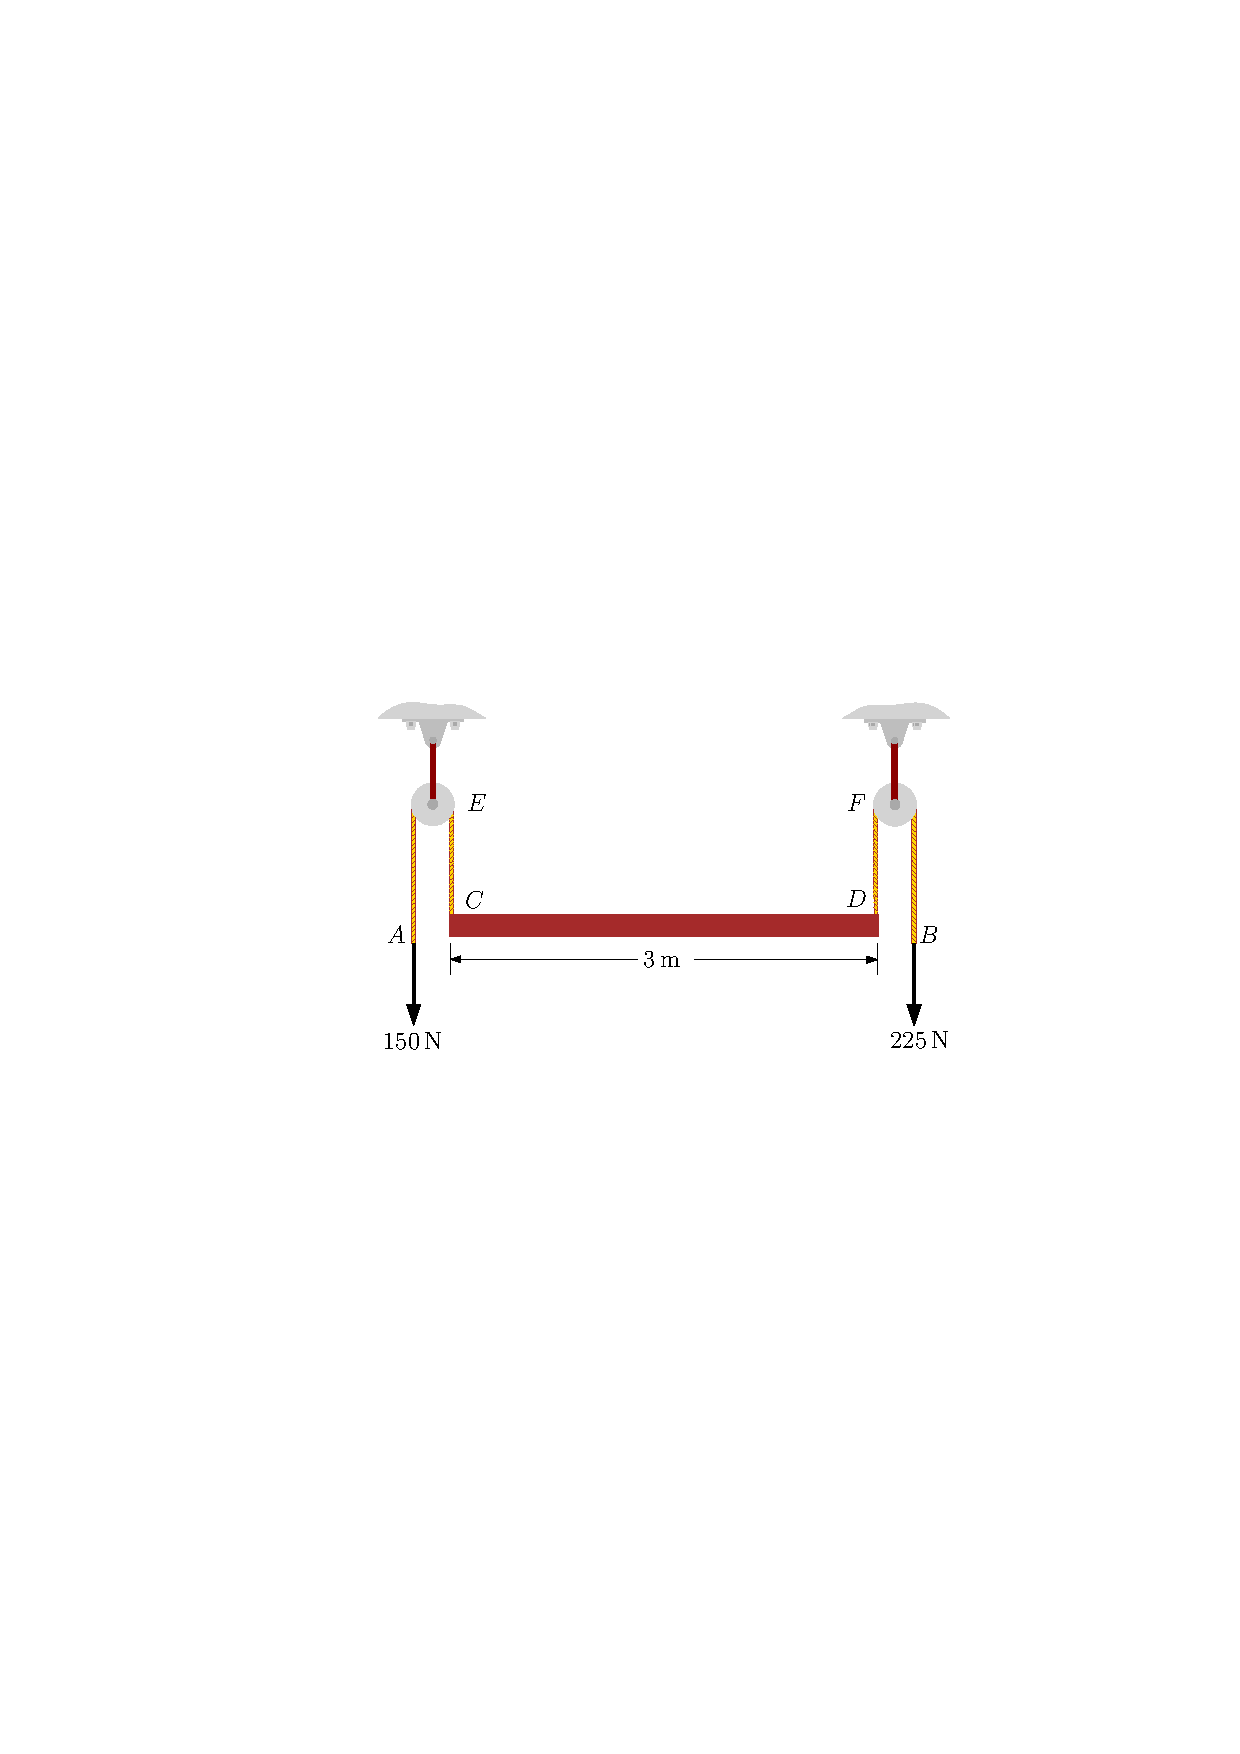
\includegraphics[scale=1]{../../images/draw_10}
\end{flushright}